

\begin{frame}{Multi-Review Summarization}
  Sei $R= \{x_i \}$ ein Datensatz von Bewertungen mit einzelnen Bewertungen $x=(x_1,...,x_{\| x \|})$, die aus einer Sequenz aus Tokens bestehen.
Ziel ist es für ein gegebenes Produkt $p$ und die entsprechenden Bewertungen $R_p \subseteq R$ eine Zusammenfassung $s_p$ zu generieren, die alle relevanten Informationen faktisch korrekt repräsentiert.
\begin{itemize}   
  \item Extraktive Modelle: \begin{itemize}
    \item LexRank (TF-IDF gewichteter Graph)
  \end{itemize}
  \item Abstraktive Modelle (VAE): \begin{itemize}
    \item MeanSum \begin{itemize}
      \item $z_p = \bar{z} \text{, mit } z=\{z_{p_1},z_{p_2},...z_{p_k}\}$
    \end{itemize}
    \item CopyCat \begin{itemize}
      \item GRU Encoder und Decoder
      \item Latentvektor $c$ für Semantik einer Reviewgruppe
    \end{itemize}
    \item Convex Aggregation for Opinion Summarization (COOP)
  \end{itemize}
\end{itemize}
\end{frame}

\begin{frame}{Convex Aggregation for Opinion Summarization}
  \begin{itemize}
    \item Untersucht unterschiedliche Kombinationen von einzelnen Latentvektoren
    \item Bewertungen, die aus den normalen Durchschnittslatentvektoren errechnet wurden ähneln sich oft
    \item Normaler Durchschnittslatentvektor hat geringe $L_2$-Norm $\| z \|$
  \end{itemize}
  \begin{figure}
    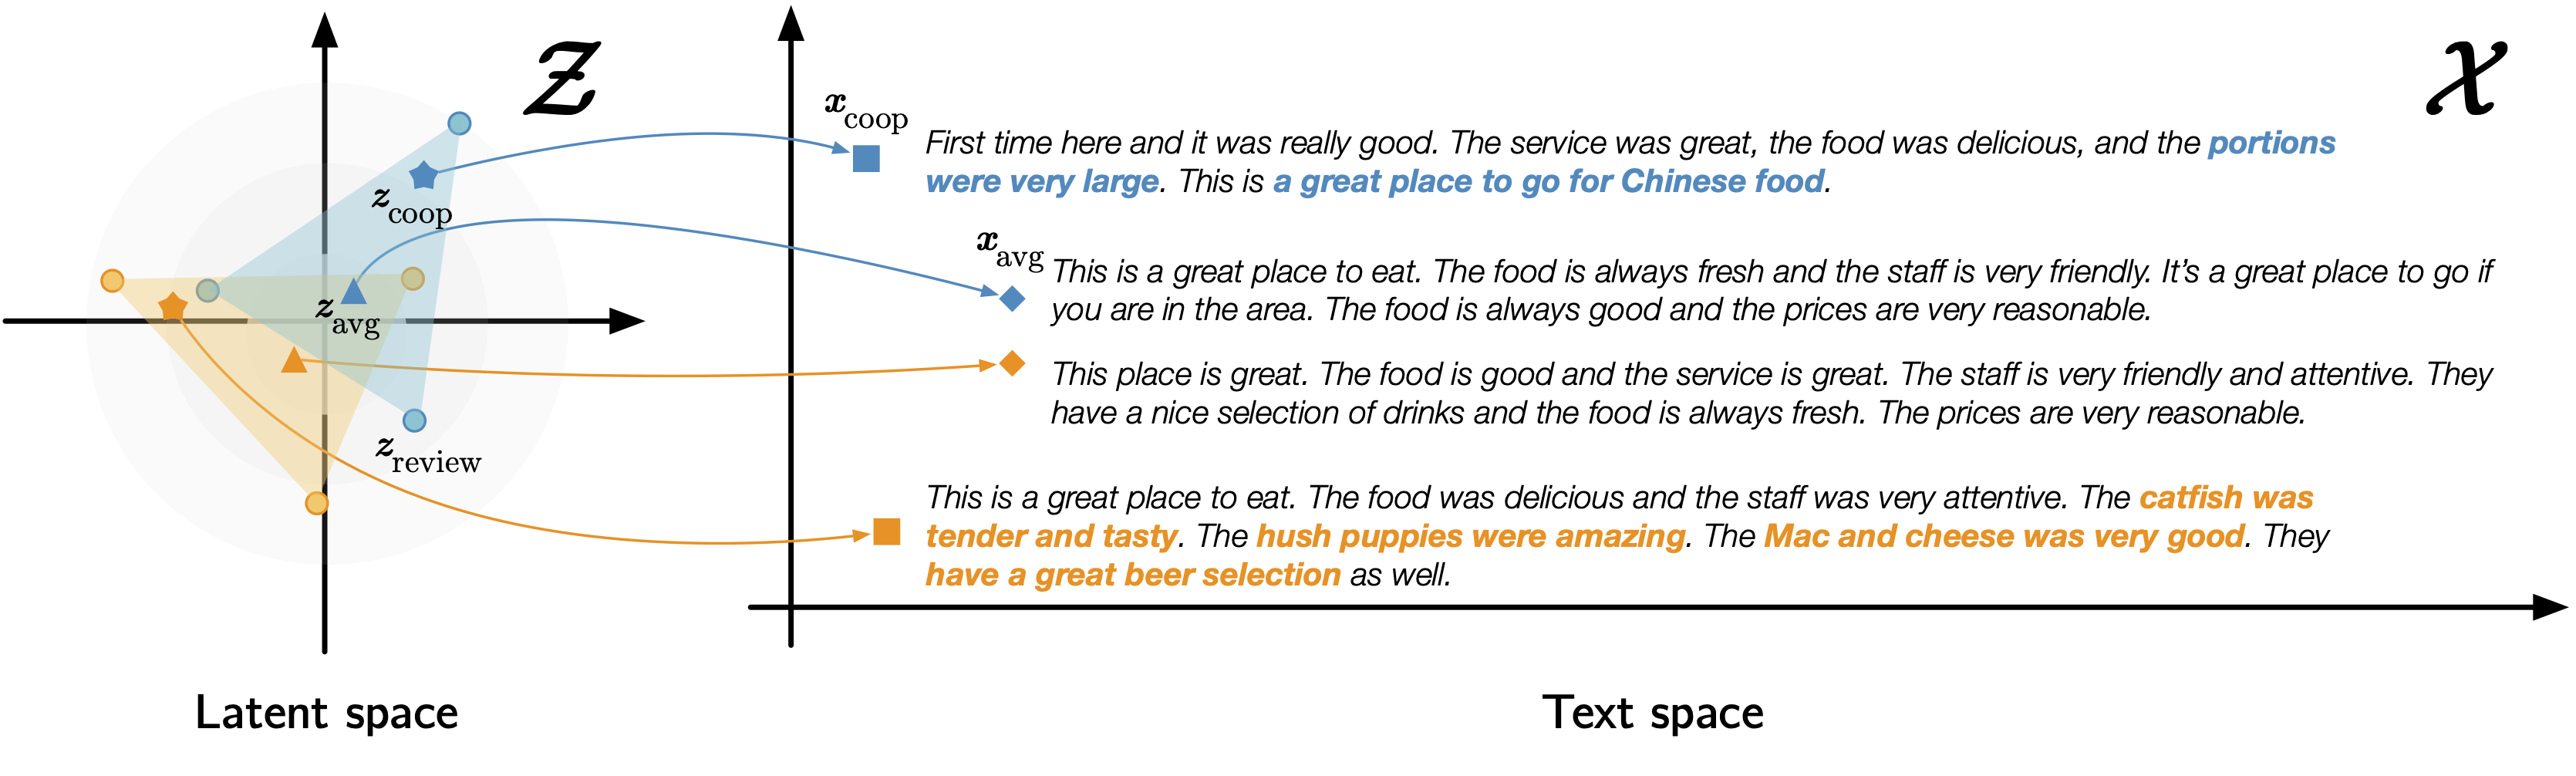
\includegraphics[width=0.85\textwidth]{bilder/coop.png}
    \caption{Latentraum Z mit den entsprechenden generierten Bewertungen X}
  \end{figure}
\end{frame}


\begin{frame}{Convex Aggregation for Opinion Summarization}
  COOP formuliert Optimierungsproblem, um die beste Kombination von einzelnen Latentvektoren zu finden:
\begin{alignat*}{2}
    \max_z              &\quad&  Overlap(R_p, D_\theta(z))    & \\
    \text{unter der Nebenbedingung: } &\quad&  z = \sum_{i=1}^{|R_p|} w_i z_i \\
                         &\quad&  \sum_{i=1}^{|R_p|}w_i=1,                        &\quad \forall w_i \in \mathbb{R}^+
\end{alignat*}

mit $Overlap(X,Y) = \text{ROUGE-1}_{F_1}(X,Y)$
\end{frame}


\begin{frame}{Convex Aggregation for Opinion Summarization}
  Suche der einzelnen Kombinationen wird auf die Potenzmenge der Eingabebewertungen $R_p$ beschränkt. 
\begin{align*}
z_p = \frac{1}{|R_p^{'}|} \sum_{i=1}^{R_p^{'}}z_i \text{, mit } R_p^{'} \in 2^{R_p} \setminus  \{ \emptyset\} 
\end{align*}

\begin{itemize}
\item ausdrucksstarke Latentvektoren
\item aktuell State-of-the-Art Ergebnisse
\item höherer Informationsgehalt als Standard Durchschnittslatentvektoren
% \item weitere Optimierungen in dieser Masterarbeit $\Rightarrow$
% \begin{itemize}
%   \item Latentvektoren adaptieren für höheres Input-Output-Overlap
%   \item neue Input-Output-Overlap Ranking Funktion
% \end{itemize}
\end{itemize}
\end{frame}



%MORE GRUNDLAGEN